%!TEX root = ../per_st_tk.tex

\begin{frame}{Steenrod construction}
	\pause
	Unlike the diagonal of spaces, chain approxs to it are \textbf{not} invariant under
	\[
	x \otimes y \stackrel{T}{\mapsto} y \otimes x.
	\]
	For example in $\gchains(\gcube) \to \gchains(\gcube) \ot \gchains(\gcube)$ we have
	\begin{center}
		\begin{tikzpicture}
		\draw[color=pblue, thick] (0,0)--(1,1);
		\draw[->] (1.25, .5) -- (1.75, .5);
		\end{tikzpicture}
		\begin{tikzpicture}
		\node at (-0.1, 1){};
		\draw[color=pblue, thick] (0,0)--(1,0)--(1,1);
		\draw (1,1)--(0,1)--(0,0);
		\end{tikzpicture}
	\end{center}

	\smallskip\pause
	To correct homotopically the breaking of this symmetry, Steenrod introduced \textbf{explicit} maps
	\[
	\Delta_i \colon \gchains(\gsimplex^n) \to \gchains(\gsimplex^n)^{\otimes 2}
	\quad \text{satisfying} \quad
	\partial \Delta_{i} = \big(1 \pm T \big) \Delta_{i-1},
	\]
	the cup-$i$ coproducts.

	\smallskip\pause
	These define the Steenrod squares as
	\[
	\begin{split}
		\Sq^k \colon H^\bullet(X; \Ftwo) &\to H^\bullet(X; \Ftwo) \\
		[\alpha] &\mapsto \big[ (\alpha \otimes \alpha) \Delta_i(-) \big]
	\end{split}
	\]
\end{frame}

\begin{frame}{Self-intersections}
	\pause
	Using Poincar\'e duality, squares measure \colorit{self-intersections} in certain cases.

	\pause\bigskip
	For example
	\begin{figure}
		\newcommand*{\xMin}{0}%
\newcommand*{\xMax}{4}%
\newcommand*{\yMin}{0}%
\newcommand*{\yMax}{4}%
\begin{center}
	\centering
	\begin{tikzpicture}[scale=.6]
		\draw[-{Latex[length=2mm]}] (-.5,\yMin)--(-.5,\yMax);
		\draw[-{Latex[length=2mm]}] (-.5,\yMin)--(-.5,\yMax-.5);
		\draw[-{Latex[length=2mm]}] (4.5,\yMin)--(4.5,\yMax);
		\draw[-{Latex[length=2mm]}] (4.5,\yMin)--(4.5,\yMax-.5);

		\draw[-{Latex[length=2mm]}] (\xMin, -.5)--(\xMax, -.5);
		\draw[-{Latex[length=2mm]}] (\xMin, 4.5)--(\xMax, 4.5);

		\draw (0,0)--(0,4)--(4,4)--(4,0)--(0,0);

		\draw[color=blue!50, very thick] (0,2) .. controls (1,2.5) and (3,1.5) .. (4,2);
		\draw[color=red!50, very thick] (0,1) .. controls (1,1.3) and (3,1) .. (4,1);

		\node at (2,5.3){Torus};
		\node at (2,-1.3){$\rank \Sq^1 = 0$};
	\end{tikzpicture}
	\hspace*{2cm}
	\begin{tikzpicture}[scale=.6]
		\draw[-{Latex[length=2mm]}] (-.5,\yMin)--(-.5,\yMax);
		\draw[-{Latex[length=2mm]}] (-.5,\yMin)--(-.5,\yMax-.5);
		\draw[-{Latex[length=2mm]}] (4.5,\yMax)--(4.5,\yMin);
		\draw[-{Latex[length=2mm]}] (4.5,\yMax)--(4.5,\yMin+.5);

		\draw[-{Latex[length=2mm]}] (\xMin, -.5)--(\xMax, -.5);
		\draw[-{Latex[length=2mm]}] (\xMin, 4.5)--(\xMax, 4.5);

		\draw (0,0)--(0,4)--(4,4)--(4,0)--(0,0);

		\draw[color=blue!50, very thick] (0,2) .. controls (1,2.5) and (3,1.5) .. (4,2);
		\draw[color=red!50, very thick] (0,1) .. controls (1,1) and (2,2.5) .. (4,3);

		\node at (2,5.3){Klein Bottle };
		\node at (2,-1.3){$\rank \Sq^1 = 1$};
	\end{tikzpicture}
%	\caption{Klein Bottle. $\rank \Sq^1 = 0$}
\end{center}
	\end{figure}

	\smallskip
	({\small a}) $\rank \big( \Sq^1\colon H^1(\rT; \Ftwo) \to H^2(\rT; \Ftwo) \big) = 0$,

	\medskip
	({\small b}) $\rank \big( \Sq^1\colon H^1(\rK; \Ftwo) \to H^2(\rK; \Ftwo) \big) = 1$.
\end{frame}

\begin{frame}[fragile]{A new description of Steenrod's construction}
	\pause
	\colorit{Notation:}
	\[
	d_u[v_0, \dots, v_m] = [v_0, \dots, \widehat v_u, \dots, v_m]
	\]
	\pause\vspace*{-15pt}
	\[
	\rP_q^n = \set[\big]{U \subseteq \{0, \dots, n\} : \bars{U} = q}
	\]
	\pause\vspace*{-15pt}
	\[
	\forall \, U = \{u_1 < \dots < u_q\} \in \rP_q^n
	\]
	\pause\vspace*{-15pt}
	\[
	d_U = d_{u_1} \dotsm \, d_{u_q}
	\]
	\pause\vspace*{-15pt}
	\[
	U^\varepsilon = \big\{ u_i \in U \mid u_i + i \equiv \varepsilon \text{ mod } 2 \big\}
	\]

	\bigskip\pause
	\colorit{Definition (Med.)} \\
	For a basis element $x \in \gchains_m(\gsimplex^n, \Ftwo)$
	\vspace*{-5pt}
	\[
	\Delta_i(x) \ = \!\!\! \sum_{U \in \rP_{m-i}^n} \!\! d_{U^0}(x) \otimes d_{U^1}(x)
	\]
	\vspace*{-10pt}

	\pause
	\colorit{Example:}
	\vspace*{-5pt}
	\begin{align*}
	\Delta_0 [0,1,2] &=
	\Big( d_{12} \otimes \id + d_2 \otimes d_0 + \id \otimes d_{01} \Big) [0,1,2]^{\otimes 2} \\ &=
	[0] \otimes [0,1,2] + [0,1] \otimes [1,2] + [0,1,2] \otimes [2].
	\end{align*}
\end{frame}

\begin{frame}{Fast computation of Steenrod squares}
	\pause
	Comparing with SAGE: (algorithm based on EZ-AW contraction)

	\smallskip\pause
	\colorit{$\Sq^1$} on \colorit{$\Sigma^i\R P^2$} ($i^\th$ suspension of the real projective plane)

	\medskip
	\includegraphics[width=\textwidth]{aux/comp_sus_rp2.pdf}
\end{frame}

\begin{frame}{Steenrod squares for simplicial complexes}
	\begin{algorithm} [H]
	\KwIn{$A = \{a_1, \dots, a_m\} \subseteq X_n$}
	$B = \emptyset$ \\
	\ForAll{$a_i\ \mathrm{and}\ a_j\ \mathrm{with}\ i < j$}
	{
		$a_{ij} = a_i \cup a_j$ \\
		\If{$a_{ij} \in X_{n+k}$}
		{
			$\overline{a}_i = a_i \setminus a_j$\ ;\ \
			$\overline{a}_j = a_j \setminus a_i$\ ;\ \
			$\overline{a}_{ij} = \overline{a}_i \cup \overline{a}_j$ \\
			$index \colon \overline{a}_{ij} \to \{0,1\}$ \\
			\ForAll {$v \in \overline{a}_{ij}$}
			{
				$p = \mathrm{position\ of\ } v \mathrm{\ in\ } a_{ij}$\ ;\ \
				$\overline{p} = \mathrm{position\ of\ } v \mathrm{\ in\ } \overline{a}_{ij}$\\
				$index(v) = {p}\, +\, \overline{p}\ \ \mathrm{residue\ mod}\ 2$
			}
			\If{\hspace*{3pt}$index(\overline{a}_i) \xor index(\overline{a}_j)$ = $\{0,1\}$}
			{$B = B \xor \{a_{ij}\}$}
		}
	}
	\KwOut{$B$}
\end{algorithm}
\end{frame}

\begin{frame}[fragile]{Steenrod barcodes}
	\pause
	Given a filtered simplicial complex $X$
	\[
	X_0 \to X_1 \to \cdots \to X_n.
	\]

	\pause
	Cohomology induces a \colorit{persistent module}, its \colorit{barcode} is a summary of how Betti numbers are consecutively shared.\\

	\smallskip
	\phantom{A cohomology operation induces an endomorphism}
	\[
	\begin{tikzcd}[column sep = 15]
		H^\bullet(X_n; \Ftwo) \arrow[r] & \cdots \arrow[r] & H^\bullet(X_{n-1}; \Ftwo) \arrow[r] & H^\bullet(X_0; \Ftwo) \\
		\phantom{H^\bullet(X_n; \Ftwo)} \arrow[u, "\phantom{\Sq^k}", phantom] & \phantom{\cdots} & \phantom{H^\bullet(X_{n-1}; \Ftwo)} & \phantom{H^\bullet(X_0; \Ftwo)} \arrow[u, "\phantom{\Sq^k}", phantom] \phantom{.}
	\end{tikzcd}
	\]
\end{frame}

\begin{frame}[fragile]{Steenrod barcodes}
	Given a filtered simplicial complex $X$
	\[
	X_0 \to X_1 \to \cdots \to X_n.
	\]
	Cohomology induces a \colorit{persistent module}, its \colorit{barcode} is a summary of how Betti numbers are consecutively shared.

	\smallskip
	A cohomology operation induces an \colorit{endomorphism}
	\[
	\begin{tikzcd}[column sep = 15]
	H^\bullet(X_n; \Ftwo) \arrow[r] & \cdots \arrow[r] & H^\bullet(X_{n-1}; \Ftwo) \arrow[r] & H^\bullet(X_0; \Ftwo) \\
	H^\bullet(X_n; \Ftwo) \arrow[u, "\Sq^k"] \arrow[r] & \cdots \arrow[r] & H^\bullet(X_{n-1}; \Ftwo) \arrow[u, "\Sq^k"] \arrow[r] & H^\bullet(X_0; \Ftwo) \arrow[u, "\Sq^k"].
	\end{tikzcd}
	\]

	\pause
	\colorit{Definition (Lupo--Med.--Tauzin)} \\
	The \colorit{$\Sq^k$-barcode} of $X$ is defined as the barcode of $\mathrm{img}\ \Sq^k$.

	\pause\medskip
	\colorit{Theorem (Ling Zhou--Med.--M\'emoli)} \\
	These barcodes are stable.
\end{frame}

\begin{frame}{Example} \pause
	Filtrations of the cone on the suspension of $S^2 \vee S^4$ and $\bC \rP^2$.

	\pause
	\begin{figure}
		\centering
		\begin{subfigure}[b]{0.49\textwidth}
			\centering
			\includegraphics[width=\textwidth]{aux/s2_s4.pdf}
			\caption{$\mathrm C\,\Sigma(S^2 \vee S^4)$}
			\label{f:s2_s4}
		\end{subfigure}
		\begin{subfigure}[b]{0.49\textwidth}
			\centering
			\includegraphics[width=\textwidth]{aux/cp2.pdf}
			\caption{$\mathrm C\,\Sigma\,\bC\rP^2$}
			\label{f:cp2}
		\end{subfigure}
	\end{figure}
\end{frame}

\begin{frame}{Algorithm}
	\pause
	It has three steps:

	\begin{enumerate}
		\pause\bigskip
		\item Usual reduction applied to the anti-transposed boundary $M$ yielding
		\[
		R = M V
		\]
		where $R$ is reduced and $V$ is invertible.

		\pause\bigskip
		\item Read off cohomology representatives and apply the new $\Sq^k$ algorithm to create a matrix $Q^k$ with the resulting representatives.

		\pause\bigskip
		\item Using that $R$ is made of generating coboundaries, apply a reduction algorithm to $Q^k$ with respect to $R$ recording the rank of $Q_{\leq j}^k$.
	\end{enumerate}
\end{frame}

\begin{frame}{Third step}
	\begin{algorithm}[H]
	\KwIn{$R,\, Q^k$}
	Alive $= \{0, \dots, m\}$,
	Barcode $= \emptyset$ \\
	\For{$j = 0, \dots, m$}{
		$R_{\leq j} \mid Q^k_{\leq j} = \text{Reduce}\left( R_{\leq j} \mid Q^k_{\leq j} \right)$ \\
		\For{$i = 0, \dots, j$}{
			\If{$i \in \mathrm{Alive\ and\ } Q^k_i = 0$}{
				remove $i$ from Alive \\
				\If{$i <j $}{add $[m-j, m-i]$ to Barcode}
			}
		}
	}
	\For{$i \in \mathrm{Alive}$}{
		add $[-1, m-i]$ to Barcode
	}
	\KwOut{Barcode}
\end{algorithm}
\end{frame}

\begin{frame}{\texttt{steenroder}}
	\pause
	With \textit{U. Lupo} and \textit{G.~Tauzin}

	\begin{center}
		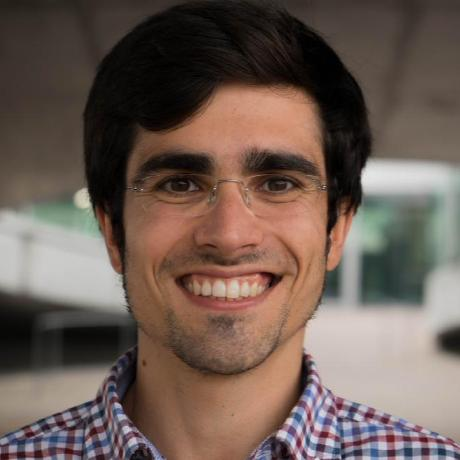
\includegraphics[scale=.2]{aux/umberto}
		\qquad
		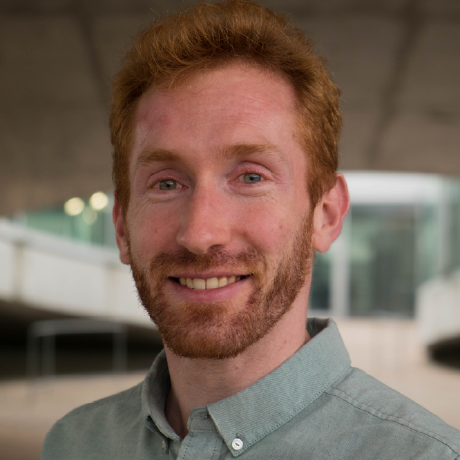
\includegraphics[scale=.2]{aux/guillaume}
	\end{center}

	from \colorit{\texttt{giotto-tda}}'s team we developed a Python package for this.

	\pause\smallskip
	It can easily installed via
	\begin{center}
		\texttt{python -m pip install -U steenroder}
	\end{center}

	and we accept contributions at
	\begin{center}
		\url{https://github.com/Steenroder/steenroder}
	\end{center}
\end{frame}

\begin{frame}{Space of conformations of $\mathrm{C_8H_{16}}$}
	\pause
	Points in $\R^{24}$ (positions of $8$ carbons in $\R^3$)

	\pause\smallskip
	Computing $\Sq^1$ barcode of a ``smooth component'' of this point cloud
	\smallskip
	\includegraphics[width=\textwidth]{aux/cyclo-octane_subsampled_absolute_barcodes.pdf}
	Consistent with a \colorit{Klein bottle} component.
\end{frame}

%\begin{frame}{Unicity of Steenrod's cup-$i$ construction}
%	\pause
%	\colorit{Theorem (Med.)} \\
%	All cup-$i$ constructions in the literature are equal up isomorphism:
%	\vskip -7.5pt
%	\[
%	\triangle \sim \triangle^\prime \iff \forall i \in \N, \ \triangle_i = \triangle_i^\prime \ \vee \, \triangle_i = T \triangle_i^\prime.
%	\]
%	\vskip -3pt
%	(Proven via an axiomatic characterization.)
%
%	\medskip\pause
%	\colorit{Theorem (Laplante-Anfossi--Med.--Vallette)} \\
%	Let $P \subset \R^n$ be an $n$-dim convex polytope.
%	A generic orthogonal ordered basis of $\R^n$ defines a cellular cup-$i$ construction $S^\infty \times P \to P \times P$.
%\end{frame}